% GNUPLOT: LaTeX picture with Postscript
\begingroup
  \makeatletter
  \providecommand\color[2][]{%
    \GenericError{(gnuplot) \space\space\space\@spaces}{%
      Package color not loaded in conjunction with
      terminal option `colourtext'%
    }{See the gnuplot documentation for explanation.%
    }{Either use 'blacktext' in gnuplot or load the package
      color.sty in LaTeX.}%
    \renewcommand\color[2][]{}%
  }%
  \providecommand\includegraphics[2][]{%
    \GenericError{(gnuplot) \space\space\space\@spaces}{%
      Package graphicx or graphics not loaded%
    }{See the gnuplot documentation for explanation.%
    }{The gnuplot epslatex terminal needs graphicx.sty or graphics.sty.}%
    \renewcommand\includegraphics[2][]{}%
  }%
  \providecommand\rotatebox[2]{#2}%
  \@ifundefined{ifGPcolor}{%
    \newif\ifGPcolor
    \GPcolorfalse
  }{}%
  \@ifundefined{ifGPblacktext}{%
    \newif\ifGPblacktext
    \GPblacktexttrue
  }{}%
  % define a \g@addto@macro without @ in the name:
  \let\gplgaddtomacro\g@addto@macro
  % define empty templates for all commands taking text:
  \gdef\gplbacktext{}%
  \gdef\gplfronttext{}%
  \makeatother
  \ifGPblacktext
    % no textcolor at all
    \def\colorrgb#1{}%
    \def\colorgray#1{}%
  \else
    % gray or color?
    \ifGPcolor
      \def\colorrgb#1{\color[rgb]{#1}}%
      \def\colorgray#1{\color[gray]{#1}}%
      \expandafter\def\csname LTw\endcsname{\color{white}}%
      \expandafter\def\csname LTb\endcsname{\color{black}}%
      \expandafter\def\csname LTa\endcsname{\color{black}}%
      \expandafter\def\csname LT0\endcsname{\color[rgb]{1,0,0}}%
      \expandafter\def\csname LT1\endcsname{\color[rgb]{0,1,0}}%
      \expandafter\def\csname LT2\endcsname{\color[rgb]{0,0,1}}%
      \expandafter\def\csname LT3\endcsname{\color[rgb]{1,0,1}}%
      \expandafter\def\csname LT4\endcsname{\color[rgb]{0,1,1}}%
      \expandafter\def\csname LT5\endcsname{\color[rgb]{1,1,0}}%
      \expandafter\def\csname LT6\endcsname{\color[rgb]{0,0,0}}%
      \expandafter\def\csname LT7\endcsname{\color[rgb]{1,0.3,0}}%
      \expandafter\def\csname LT8\endcsname{\color[rgb]{0.5,0.5,0.5}}%
    \else
      % gray
      \def\colorrgb#1{\color{black}}%
      \def\colorgray#1{\color[gray]{#1}}%
      \expandafter\def\csname LTw\endcsname{\color{white}}%
      \expandafter\def\csname LTb\endcsname{\color{black}}%
      \expandafter\def\csname LTa\endcsname{\color{black}}%
      \expandafter\def\csname LT0\endcsname{\color{black}}%
      \expandafter\def\csname LT1\endcsname{\color{black}}%
      \expandafter\def\csname LT2\endcsname{\color{black}}%
      \expandafter\def\csname LT3\endcsname{\color{black}}%
      \expandafter\def\csname LT4\endcsname{\color{black}}%
      \expandafter\def\csname LT5\endcsname{\color{black}}%
      \expandafter\def\csname LT6\endcsname{\color{black}}%
      \expandafter\def\csname LT7\endcsname{\color{black}}%
      \expandafter\def\csname LT8\endcsname{\color{black}}%
    \fi
  \fi
    \setlength{\unitlength}{0.0500bp}%
    \ifx\gptboxheight\undefined%
      \newlength{\gptboxheight}%
      \newlength{\gptboxwidth}%
      \newsavebox{\gptboxtext}%
    \fi%
    \setlength{\fboxrule}{0.5pt}%
    \setlength{\fboxsep}{1pt}%
\begin{picture}(5000.00,5000.00)%
    \gplgaddtomacro\gplbacktext{%
      \colorrgb{0.15,0.15,0.15}%
      \put(518,2997){\makebox(0,0)[r]{\strut{}\small $0.02$}}%
      \colorrgb{0.15,0.15,0.15}%
      \put(518,3268){\makebox(0,0)[r]{\strut{}\small $0.03$}}%
      \colorrgb{0.15,0.15,0.15}%
      \put(518,3539){\makebox(0,0)[r]{\strut{}\small $0.04$}}%
      \colorrgb{0.15,0.15,0.15}%
      \put(518,3811){\makebox(0,0)[r]{\strut{}\small $0.05$}}%
      \colorrgb{0.15,0.15,0.15}%
      \put(518,4082){\makebox(0,0)[r]{\strut{}\small $0.06$}}%
      \colorrgb{0.15,0.15,0.15}%
      \put(518,4353){\makebox(0,0)[r]{\strut{}\small $0.07$}}%
      \colorrgb{0.15,0.15,0.15}%
      \put(518,4624){\makebox(0,0)[r]{\strut{}\small $0.08$}}%
      \colorrgb{0.15,0.15,0.15}%
      \put(832,2777){\makebox(0,0){\strut{}\small FSMSM}}%
      \colorrgb{0.15,0.15,0.15}%
      \put(1414,2777){\makebox(0,0){\strut{}\small CSM}}%
      \colorrgb{0.15,0.15,0.15}%
      \put(1895,2777){\makebox(0,0){\strut{}\small NDT}}%
    }%
    \gplgaddtomacro\gplfronttext{%
      \colorrgb{0.00,0.00,0.00}%
      \put(1413,4844){\makebox(0,0){\strut{}$\sigma_R = 0.01$ m}}%
    }%
    \gplgaddtomacro\gplbacktext{%
      \colorrgb{0.15,0.15,0.15}%
      \put(2865,2997){\makebox(0,0)[r]{\strut{}\small $0.02$}}%
      \colorrgb{0.15,0.15,0.15}%
      \put(2865,3229){\makebox(0,0)[r]{\strut{}\small $0.03$}}%
      \colorrgb{0.15,0.15,0.15}%
      \put(2865,3462){\makebox(0,0)[r]{\strut{}\small $0.04$}}%
      \colorrgb{0.15,0.15,0.15}%
      \put(2865,3694){\makebox(0,0)[r]{\strut{}\small $0.05$}}%
      \colorrgb{0.15,0.15,0.15}%
      \put(2865,3927){\makebox(0,0)[r]{\strut{}\small $0.06$}}%
      \colorrgb{0.15,0.15,0.15}%
      \put(2865,4159){\makebox(0,0)[r]{\strut{}\small $0.07$}}%
      \colorrgb{0.15,0.15,0.15}%
      \put(2865,4392){\makebox(0,0)[r]{\strut{}\small $0.08$}}%
      \colorrgb{0.15,0.15,0.15}%
      \put(3179,2777){\makebox(0,0){\strut{}\small FSMSM}}%
      \colorrgb{0.15,0.15,0.15}%
      \put(3761,2777){\makebox(0,0){\strut{}\small CSM}}%
      \colorrgb{0.15,0.15,0.15}%
      \put(4242,2777){\makebox(0,0){\strut{}\small NDT}}%
    }%
    \gplgaddtomacro\gplfronttext{%
      \colorrgb{0.00,0.00,0.00}%
      \put(3760,4844){\makebox(0,0){\strut{}$\sigma_R = 0.03$ m}}%
    }%
    \gplgaddtomacro\gplbacktext{%
      \colorrgb{0.15,0.15,0.15}%
      \put(518,899){\makebox(0,0)[r]{\strut{}\small $0.05$}}%
      \colorrgb{0.15,0.15,0.15}%
      \put(518,1480){\makebox(0,0)[r]{\strut{}\small $0.10$}}%
      \colorrgb{0.15,0.15,0.15}%
      \put(518,2061){\makebox(0,0)[r]{\strut{}\small $0.15$}}%
      \colorrgb{0.15,0.15,0.15}%
      \put(832,330){\makebox(0,0){\strut{}\small FSMSM}}%
      \colorrgb{0.15,0.15,0.15}%
      \put(1414,330){\makebox(0,0){\strut{}\small CSM}}%
      \colorrgb{0.15,0.15,0.15}%
      \put(1895,330){\makebox(0,0){\strut{}\small NDT}}%
    }%
    \gplgaddtomacro\gplfronttext{%
      \colorrgb{0.00,0.00,0.00}%
      \put(1413,2397){\makebox(0,0){\strut{}$\sigma_R = 0.05$ m}}%
    }%
    \gplgaddtomacro\gplbacktext{%
      \colorrgb{0.15,0.15,0.15}%
      \put(2865,550){\makebox(0,0)[r]{\strut{}\small $0.0$}}%
      \colorrgb{0.15,0.15,0.15}%
      \put(2865,875){\makebox(0,0)[r]{\strut{}\small $0.05$}}%
      \colorrgb{0.15,0.15,0.15}%
      \put(2865,1201){\makebox(0,0)[r]{\strut{}\small $0.10$}}%
      \colorrgb{0.15,0.15,0.15}%
      \put(2865,1526){\makebox(0,0)[r]{\strut{}\small $0.15$}}%
      \colorrgb{0.15,0.15,0.15}%
      \put(2865,1852){\makebox(0,0)[r]{\strut{}\small $0.20$}}%
      \colorrgb{0.15,0.15,0.15}%
      \put(2865,2177){\makebox(0,0)[r]{\strut{}\small $0.25$}}%
      \colorrgb{0.15,0.15,0.15}%
      \put(3179,330){\makebox(0,0){\strut{}\small FSMSM}}%
      \colorrgb{0.15,0.15,0.15}%
      \put(3761,330){\makebox(0,0){\strut{}\small CSM}}%
      \colorrgb{0.15,0.15,0.15}%
      \put(4242,330){\makebox(0,0){\strut{}\small NDT}}%
    }%
    \gplgaddtomacro\gplfronttext{%
      \colorrgb{0.00,0.00,0.00}%
      \put(3760,2397){\makebox(0,0){\strut{}$\sigma_R = 0.10$ m}}%
      \put(2500,5200){\makebox(0,0){\strut{}Distributions of mean pose errors --- $\sigma_{\bm{M}} = 0.05$ m}}%
    }%
    \gplbacktext
    \put(0,0){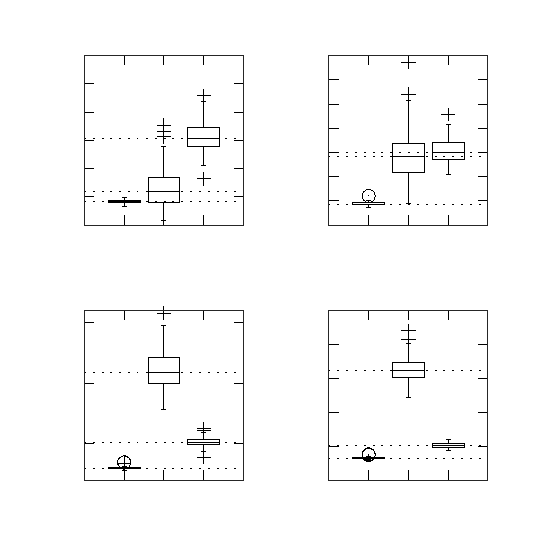
\includegraphics{./figures/experiments/boxplot_errors_CSM_KUF_NDT_sm5}}%
    \gplfronttext
  \end{picture}%
\endgroup
